\chapter{\IfLanguageName{dutch}{POC1: Simulatie}{POC1: Simulation}}%
\label{ch:poc1}

%TODO:
De eerste \gls{poc} is een simulatie van een 5G-netwerk. Dit wordt opgezet door gebruik te maken van \gls{open5gs}

\begin{figure}
    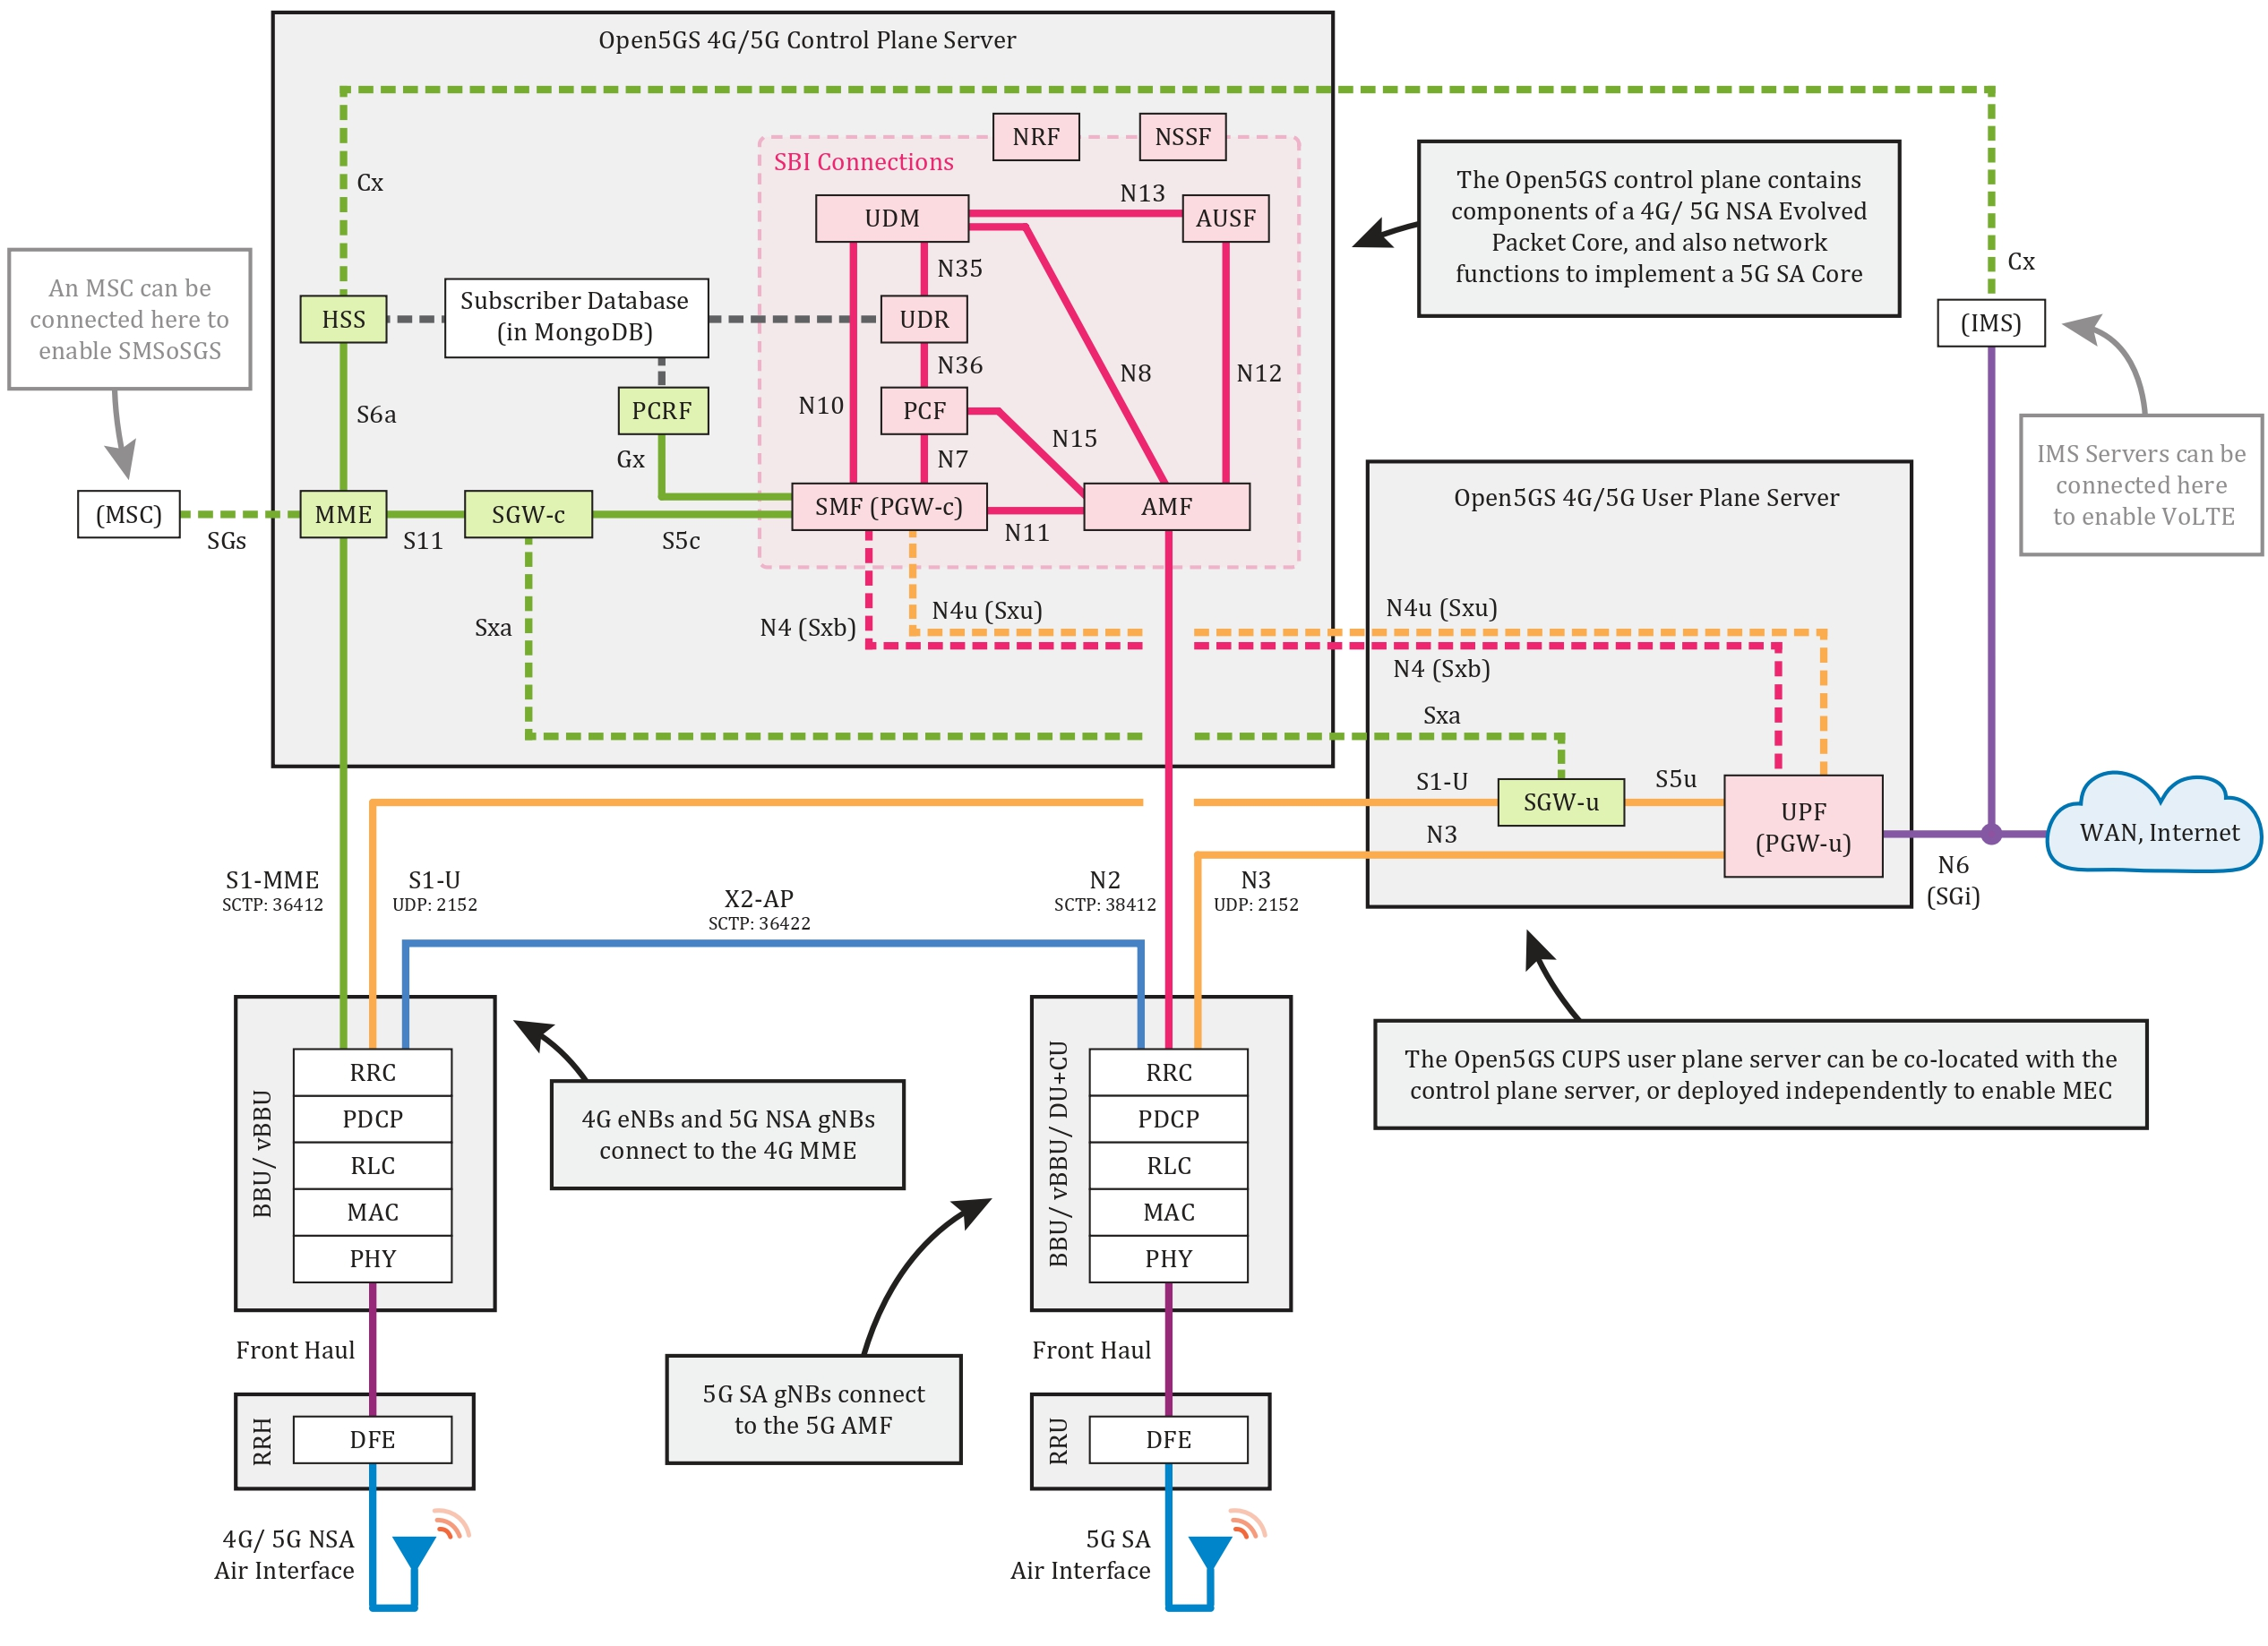
\includegraphics[width=\linewidth]{../graphics/Open5GS-Schema.jpg}
    \caption{Gesimuleerd 5G-netwerk met Open5GS. \autocite[Door][Copyright 2021 van \citeauthor{Lee2021}]{Lee2021}}
    \label{fig:open5gs-schema}
\end{figure}